\documentclass{article}

\usepackage{arxiv}

\usepackage[utf8]{inputenc} % allow utf-8 input
\usepackage[T1]{fontenc}    % use 8-bit T1 fonts
\usepackage{lmodern}        % https://github.com/rstudio/rticles/issues/343
\usepackage{hyperref}       % hyperlinks
\usepackage{url}            % simple URL typesetting
\usepackage{booktabs}       % professional-quality tables
\usepackage{amsfonts}       % blackboard math symbols
\usepackage{nicefrac}       % compact symbols for 1/2, etc.
\usepackage{microtype}      % microtypography
\usepackage{lipsum}
\usepackage{graphicx}

\title{Economies of scale: Larger vaccination distribution hubs are more
resiliant to service disruptions}

\author{
    Mark Hanly
   \\
    Centre for Big Data Research in Health \\
    UNSW Sydney \\
   \\
  \texttt{\href{mailto:m.hanly@unsw.edu.au}{\nolinkurl{m.hanly@unsw.edu.au}}} \\
   \And
    Tim Churches
   \\
    South Western Sydney Clinical School, Faculty of Medicine \& Health,
  UNSW Sydney \& \\
    Ingham Institute for Applied Medical Research \\
   \\
  \texttt{\href{mailto:timothy.churches@unsw.edu.au}{\nolinkurl{timothy.churches@unsw.edu.au}}} \\
   \And
    Oisín Fitzgerald
   \\
    Centre for Big Data Research in Health \\
    UNSW Sydney \\
   \\
  \texttt{\href{mailto:o.fitzgerald@unsw.edu.au}{\nolinkurl{o.fitzgerald@unsw.edu.au}}} \\
   \And
    Ian Caterson
   \\
    School of Life and Environmental Sciences \\
    University of Sydney \\
   \\
  \texttt{\href{mailto:ian.caterson@sydney.edu.au}{\nolinkurl{ian.caterson@sydney.edu.au}}} \\
   \And
    Chandini Raina MacIntyre
   \\
    Biosecurity Research Program, The Kirby Institute \\
    UNSW Sydney \\
   \\
  \texttt{\href{mailto:rainam@protonmail.com}{\nolinkurl{rainam@protonmail.com}}} \\
   \And
    Louisa Jorm
   \\
    Centre for Big Data Research in Health \\
    UNSW Sydney \\
   \\
  \texttt{\href{mailto:l.jorm@unsw.edu.au}{\nolinkurl{l.jorm@unsw.edu.au}}} \\
  }


% Pandoc citation processing

\usepackage{float}
\usepackage{booktabs}
\usepackage{longtable}
\usepackage{array}
\usepackage{multirow}
\usepackage{wrapfig}
\usepackage{colortbl}
\usepackage{pdflscape}
\usepackage{tabu}
\usepackage{threeparttable}
\usepackage{threeparttablex}
\usepackage[normalem]{ulem}
\usepackage{makecell}
\usepackage{xcolor}


\begin{document}
\maketitle

\def\tightlist{}


\begin{abstract}
Abstract to be added here
\end{abstract}

\keywords{
    COVID19
   \and
    vaccination
  }

\newpage

\hypertarget{introduction}{%
\section{Introduction}\label{introduction}}

\hypertarget{methods}{%
\section{Methods}\label{methods}}

\begin{figure}[h]

{\centering 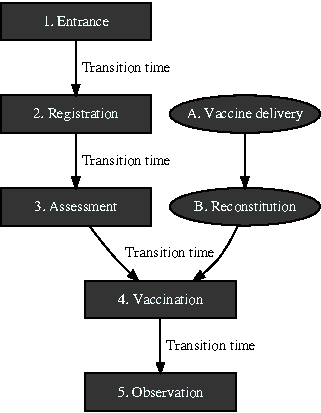
\includegraphics{Preprint_files/figure-latex/modelGraph-1} 

}

\caption{Queueing model for a vaccination site}\label{fig:modelGraph}
\end{figure}

\begin{table}[H]

\caption{\label{tab:unnamed-chunk-1}Service time parameter values and resulting distributions}
\begin{tabu} to \linewidth {>{\raggedright}X>{\raggedleft}X>{\raggedleft}X>{\raggedleft}X>{\raggedleft}X>{\raggedleft}X>{\raggedleft}X>{\raggedleft}X>{\raggedleft}X>{}l}
\toprule
\multicolumn{4}{c}{ } & \multicolumn{5}{c}{Percentiles} & \multicolumn{1}{c}{ } \\
\cmidrule(l{3pt}r{3pt}){5-9}
Station & Staff & Base time & Rate & 5\% & 25\% & 50\% & 75\% & 95\% & Distribution\\
\midrule
\cellcolor{gray!6}{Reconstitution} & \cellcolor{gray!6}{7} & \cellcolor{gray!6}{1} & \cellcolor{gray!6}{3.0} & \cellcolor{gray!6}{1.0} & \cellcolor{gray!6}{1.1} & \cellcolor{gray!6}{1.2} & \cellcolor{gray!6}{1.5} & \cellcolor{gray!6}{2.0} & \cellcolor{gray!6}{
\includegraphics[width=0.67in, height=0.17in]{Preprint_files/figure-latex//hist_ed6244e1693.pdf}}\\
Entrance & 8 & 2 & 1.0 & 2.1 & 2.3 & 2.7 & 3.3 & 5.0 & 
\includegraphics[width=0.67in, height=0.17in]{Preprint_files/figure-latex//hist_ed67249147a.pdf}\\
\cellcolor{gray!6}{Registration} & \cellcolor{gray!6}{12} & \cellcolor{gray!6}{3} & \cellcolor{gray!6}{0.5} & \cellcolor{gray!6}{3.1} & \cellcolor{gray!6}{3.6} & \cellcolor{gray!6}{4.3} & \cellcolor{gray!6}{5.7} & \cellcolor{gray!6}{9.2} & \cellcolor{gray!6}{
\includegraphics[width=0.67in, height=0.17in]{Preprint_files/figure-latex//hist_ed672745437.pdf}}\\
Assessment & 8 & 2 & 1.0 & 2.1 & 2.3 & 2.7 & 3.4 & 4.9 & 
\includegraphics[width=0.67in, height=0.17in]{Preprint_files/figure-latex//hist_ed67f9fd77e.pdf}\\
\cellcolor{gray!6}{Vaccination} & \cellcolor{gray!6}{14} & \cellcolor{gray!6}{2} & \cellcolor{gray!6}{1.0} & \cellcolor{gray!6}{2.1} & \cellcolor{gray!6}{2.3} & \cellcolor{gray!6}{2.7} & \cellcolor{gray!6}{3.4} & \cellcolor{gray!6}{5.2} & \cellcolor{gray!6}{
\includegraphics[width=0.67in, height=0.17in]{Preprint_files/figure-latex//hist_ed67069fe8e.pdf}}\\
\bottomrule
\end{tabu}
\end{table}

\hypertarget{assumed-arrival-times-for-the-baseline-model}{%
\subsection{Assumed arrival times for the baseline
model}\label{assumed-arrival-times-for-the-baseline-model}}

\begin{figure}[h]

{\centering 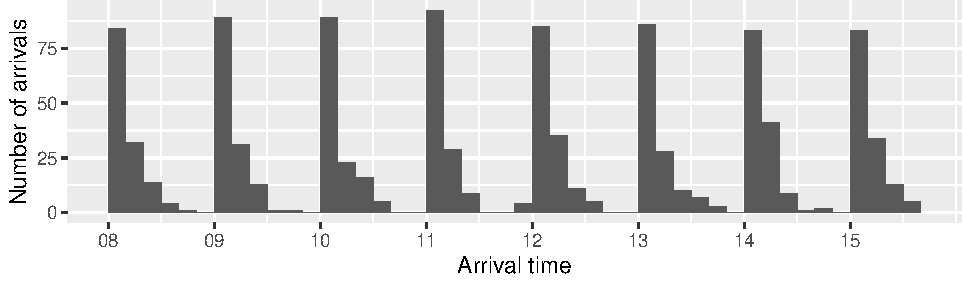
\includegraphics{Preprint_files/figure-latex/arrivalTimes-1} 

}

\caption{Example of the randomly generated arrival times, with bookings at quarter past the hour, every hour}\label{fig:arrivalTimes}
\end{figure}

\hypertarget{results}{%
\section{Results}\label{results}}

\hypertarget{staff-utilisation-factor-for-the-baseline-model}{%
\subsection{Staff utilisation factor for the baseline
model}\label{staff-utilisation-factor-for-the-baseline-model}}

\begin{figure}[h]

{\centering 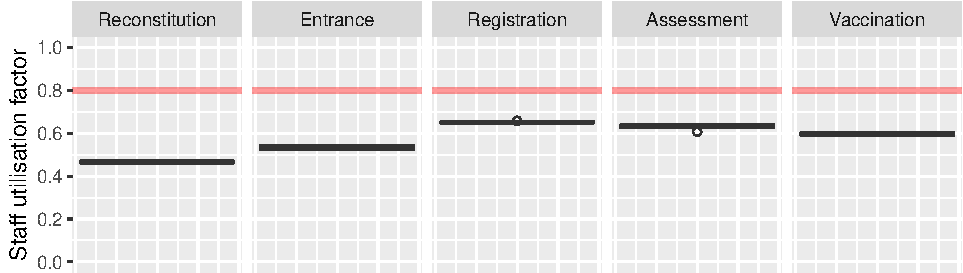
\includegraphics{Preprint_files/figure-latex/staffUtilisation-1} 

}

\caption{Processing times for the baseline model}\label{fig:staffUtilisation}
\end{figure}

\hypertarget{processing-times-for-the-baseline-model}{%
\subsection{Processing times for the baseline
model}\label{processing-times-for-the-baseline-model}}

\begin{figure}[h]

{\centering 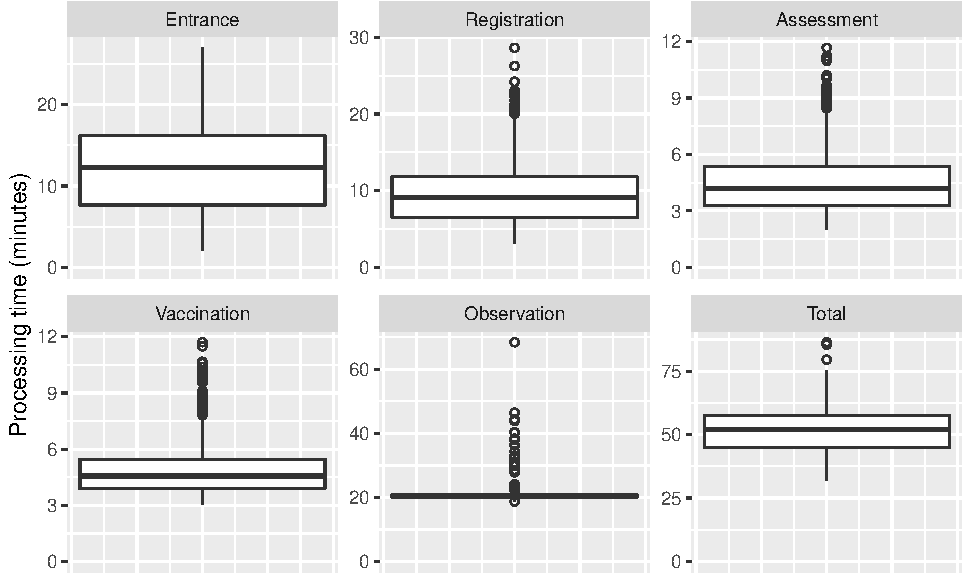
\includegraphics{Preprint_files/figure-latex/processingTimes-1} 

}

\caption{Processing times for the baseline model}\label{fig:processingTimes}
\end{figure}

\hypertarget{daily-thorughput-for-the-baseline-model}{%
\subsection{Daily thorughput for the baseline
model}\label{daily-thorughput-for-the-baseline-model}}

\begin{figure}[h]

{\centering 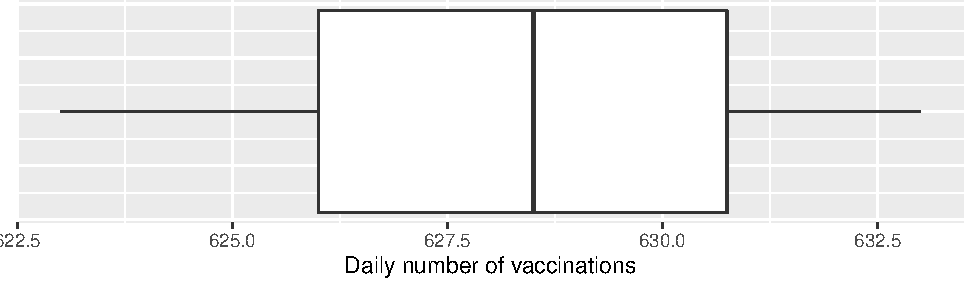
\includegraphics{Preprint_files/figure-latex/dailyThroughput-1} 

}

\caption{Daily thorughput for the baseline model}\label{fig:dailyThroughput}
\end{figure}

\hypertarget{baseline-utilisation-factor}{%
\subsection{Baseline utilisation
factor}\label{baseline-utilisation-factor}}

\begin{figure}[h]

{\centering 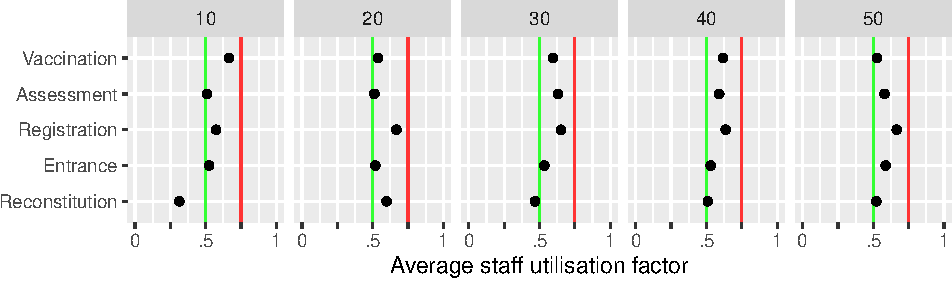
\includegraphics{Preprint_files/figure-latex/baselineUtilisation-1} 

}

\caption{Baseline staff utilisation factor}\label{fig:baselineUtilisation}
\end{figure}

\hypertarget{baseline-processing-time}{%
\subsection{Baseline processing time}\label{baseline-processing-time}}

\begin{figure}[h]

{\centering 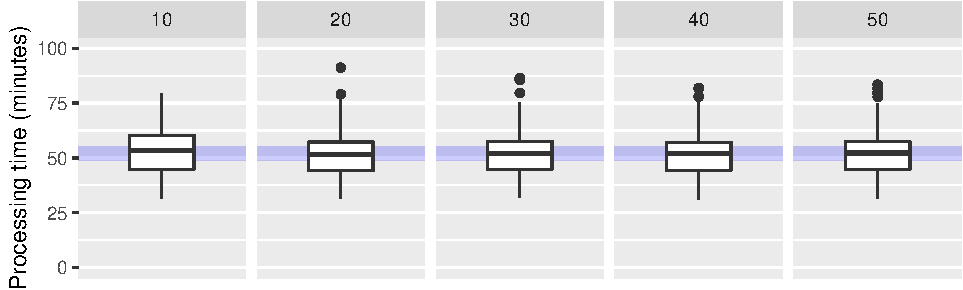
\includegraphics{Preprint_files/figure-latex/baselineProcessTime-1} 

}

\caption{Baseline processing time}\label{fig:baselineProcessTime}
\end{figure}

\hypertarget{throughput-across-larger-sites}{%
\subsection{Throughput across larger
sites}\label{throughput-across-larger-sites}}

\begin{figure}[h]

{\centering 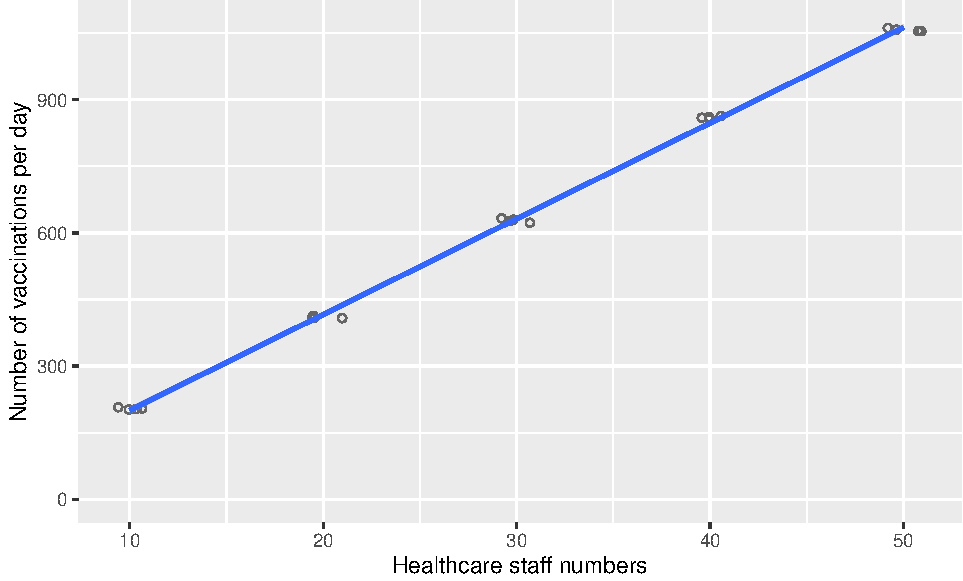
\includegraphics{Preprint_files/figure-latex/baselineThroughput-1} 

}

\caption{Baseline processing time}\label{fig:baselineThroughput}
\end{figure}

\hypertarget{increase-in-processing-time-with-increased-arrivals-by-site-size}{%
\subsection{Increase in processing time with increased arrivals by site
size}\label{increase-in-processing-time-with-increased-arrivals-by-site-size}}

\begin{figure}[h]

{\centering 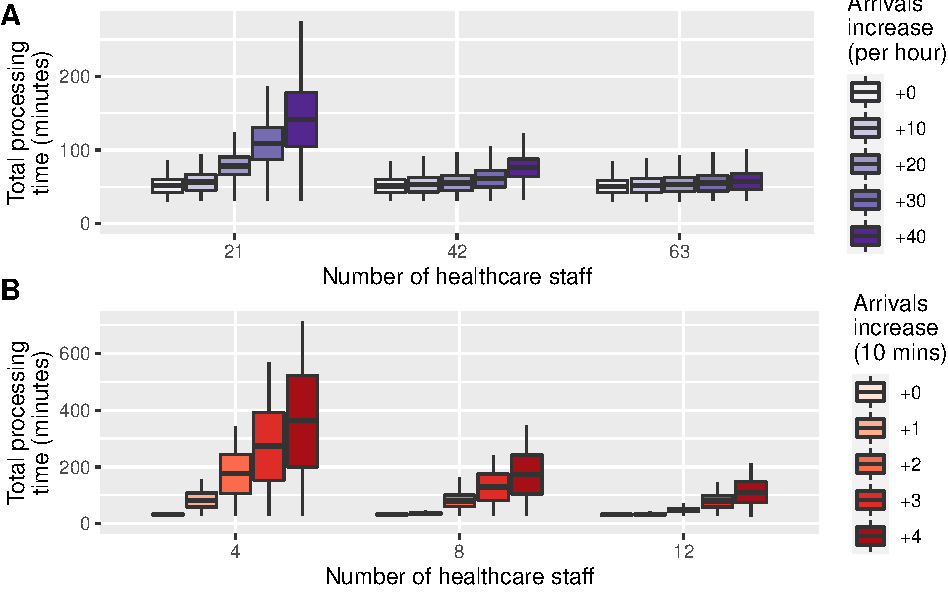
\includegraphics{Preprint_files/figure-latex/processingTimeTest-1} 

}

\caption{Increase in processing time with increased arrivals by site size}\label{fig:processingTimeTest}
\end{figure}

\hypertarget{increase-in-processing-time-with-delays-to-registration-time}{%
\subsection{Increase in processing time with delays to registration
time}\label{increase-in-processing-time-with-delays-to-registration-time}}

\begin{figure}[h]

{\centering 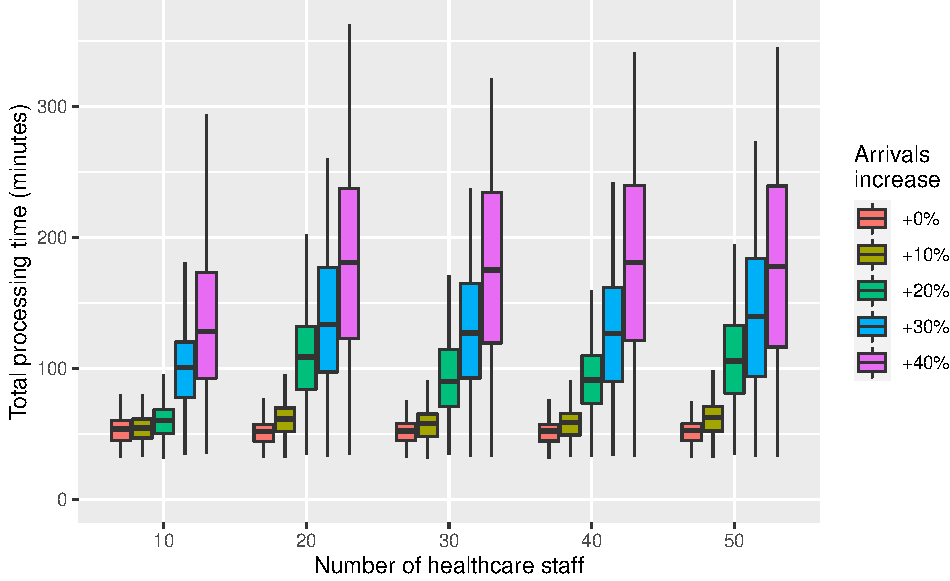
\includegraphics{Preprint_files/figure-latex/registrationTimeTest-1} 

}

\caption{Increase in processing time with increased arrivals by site size}\label{fig:registrationTimeTest}
\end{figure}

\hypertarget{discussion}{%
\section{Discussion}\label{discussion}}

\hypertarget{contributions}{%
\section{Contributions}\label{contributions}}

\hypertarget{acknowledgements}{%
\section{Acknowledgements}\label{acknowledgements}}

This research was supported by the generous assistance of Ian Sharp,
philanthropic supporter of UNSW research, and by a research seed grant
provided by the Sydney Partnership for Health, Education, Research and
Enterprise (SPHERE) Infectious diseases, Immunity and Inflammation
(Triple-I) Clinical Academic Group.

\newpage

\hypertarget{references}{%
\section{References}\label{references}}

\bibliographystyle{unsrt}
\bibliography{references.bib}


\end{document}
